\documentclass[11pt,a4paper]{article}
\usepackage[utf8]{inputenc}
%\usepackage[catalan]{babel}
\usepackage{comment}
\usepackage{amsmath}
\usepackage{amsfonts}
\usepackage{amssymb}
\usepackage{graphicx}
\usepackage{fancyhdr}
\usepackage{appendix}
\usepackage{subfig}
\usepackage[ampersand]{easylist}
\usepackage{multirow}
\usepackage[hidelinks]{hyperref}
\usepackage[left=2cm,right=2cm,top=2cm,bottom=2cm]{geometry} 


\begin{document}
\begin{titlepage}

\begin{flushleft}
Escola Politècnica Superior\\
\vspace*{0.15in}
Master of Computer Engineering\\
\vspace*{0.15in}
ICT Project: Development and Implementation
\end{flushleft}

\begin{center}
\vspace{2.0cm}
\includegraphics[scale=0.3]{figures/M-UdL.jpg}
\vspace{5.0cm}

\begin{LARGE}
\textbf{Sprint 1:}\\ 
\vspace*{0.15in}
\textbf{Requirement definition and analysis}
\end{LARGE}
\vspace{5.0cm}

\vspace*{0.25in}
\rule{80mm}{0.1mm}\\
\vspace*{0.1in}

\begin{large}
%\textbf{Teachers:} Jordi Gerv\\
\textbf{Students:}

\begin{tabular}{ll}
Roger Truchero Visa  & Gerard Donaire Alos \\
David Sarrat González  & Adrià Casals Espax \\
\multicolumn{2}{c}{Joan Pau Castells Gasia}
\end{tabular}
\\
\textbf{Date:} \today
\end{large}

\end{center}
\end{titlepage}

\lhead[\thepage]{
\includegraphics[scale=0.05]{figures/M-UdL.jpg}  }
\chead[]{\textbf{Automatic irrigation system with plague detection}}
\rhead[]{ICT Project}
\renewcommand{\headrulewidth}{0.5pt}
\renewcommand{\footrulewidth}{0.5pt}
\fancypagestyle{plain}{
\fancyhead[L]{}
\fancyhead[C]{}
\fancyhead[R]{\thepage}
\fancyfoot[L]{}
\fancyfoot[C]{}
\fancyfoot[R]{}
\renewcommand{\headrulewidth}{0pt}
\renewcommand{\footrulewidth}{0pt}
}
\pagestyle{fancy}
\vspace*{0.05in}

\tableofcontents
\vspace*{0.3in}
%\listoffigures
\newpage

\part*{Introduction}
The main idea is to design a watering system that allows us from a mobile app to water our plants remotely. This system will have different options of watering: Manual, planned and automatic sheet that the user can configure from the mobile app.\\

Additionally, we will install a plague recognition system formed by a neuronal convoluted network model that will feed images that you will receive from the webcam of the Raspberry Pi. All this information can be obtained with the option to monitor.\\

This means that we can go on vacation peacefully without having to worry about our plants and with the option to see their current status.

\newpage

\part{Sprint 1}
\section{Requirements}
\subsection{Non-functional requirements}
\begin{enumerate}
\item \textbf{Product}
	\begin{enumerate}
	
	\item \textbf{Accessibility and Usability}
		\begin{enumerate}
		\item Regardless of the style of interaction, the interface has to be simple and intuitive, providing a high level of interactivity and usability. The tasks will be as visual as possible, since the application will be oriented to all types of age ranges. 
		\end{enumerate}
	\item \textbf{Concurrency}
		\begin{enumerate}
		\item  The app has to be multi-user, allowing the usage of several users simultaneously of the application.
		\end{enumerate}
		
	\item \textbf{Portability}
		\begin{enumerate}
		\item \textbf{Adaptability (multi-device):} It is required that the design is "responsive" in order to ensure proper display on multiple devices, such as tablets, smartphones...
		\end{enumerate}
		
	\item \textbf{Support}
		\begin{enumerate}
		\item The mobile app will be developed by the Android platform.
		\end{enumerate}
	\end{enumerate}

\item \textbf{External}
	\begin{enumerate}
	\item \textbf{Privacy} 
		\begin{enumerate}
		\item All data management has to conform to the requirements of the organic law of data protection in order to preserve privacy in the processing of personal data.
		\end{enumerate}
		
	\end{enumerate}

\begin{comment}
\item \textbf{Other restrictions}
	\begin{enumerate}
	\item ??
	\end{enumerate}
\end{comment}
\end{enumerate}

\subsection{Functional requirements}
\subsection{List of functionalities and features}
\textit{List of functionalities and features that all services (Android app, web service and Arduino) will accomplish}

\subsubsection{Android app}
\begin{itemize}
\item \textbf{The Android app will have to} allow communication with the web service.

\item \textbf{The Android app will have to} allow each user to log in.

\item \textbf{The Android app will have to} allow each user to configure/create an irrigation unit independently.

\item \textbf{The Android app will have to} show all irrigation units configured by the user.

\item \textbf{The Android app will have to} allow the manual watering option for each watering unit.

\item \textbf{The Android app will have to} allow planned irrigation of each irrigation unit.

\item \textbf{The Android app will have to} allow the option of monitoring the crop with data obtained from sensors and the webcam.

\item \textbf{The Android app will have to} allow the change of language.
\end{itemize}

\subsubsection{Web service}
\begin{itemize}
\item \textbf{The web service will have to} allow communication with the Android application and the Arduino devices.

\item \textbf{The web service will have to} allow the execution of a cron to make requests to the Arduino every X time so that a user can automatically receive notifications of his crop.

\item \textbf{The web service will have to} allow the execution of a machine learning script in charge of pest detection and return the data back to the Android application.

\item \textbf{The web service will have to} be able to determine when watering is optimal (if the automatic watering function has been used without programming) and send the request to the Arduino.

\item \textbf{The web service will have to} allow CRUD operations directly from the DB.
\end{itemize}

\subsubsection{Detection plague script}
\begin{itemize}
\item \textbf{The pest detection algorithm will have to} be able to perform leaf trimming, and then pass it on to the convolutional neural network.

\item \textbf{The pest detection algorithm will have to}, using an image of a leaf as an input, determine if this is a pest or not.
\end{itemize}

\subsubsection{Arduino}
\begin{itemize}
\item \textbf{The Arduino system will have to} allow communication with the web service.

\item \textbf{The Arduino system will have to} allow images to be sent in real time to the web service.

\item \textbf{The Arduino system will have to} allow the data from the humidity, temperature and soil sensors to be captured.

\end{itemize}

\newpage

\section{Main use cases}
%% Main use cases

\section{General architecture}
\subsection{System architecture}
\begin{figure}[hbtp]
\centering
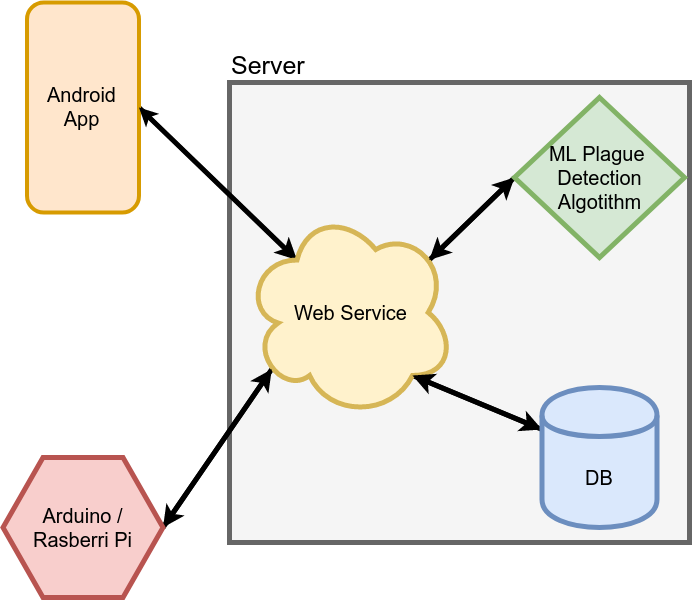
\includegraphics[scale=0.6]{figures/AppArchitecture.png}
\caption{System app architecture}
\end{figure}

\subsection{Arduino/Raspberry pi architecture}
\begin{figure}[hbtp]
\centering
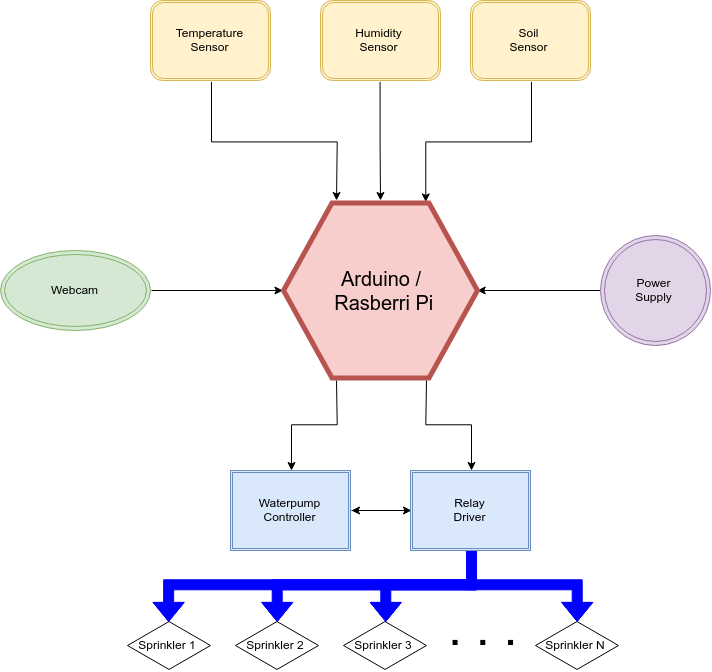
\includegraphics[scale=0.6]{figures/ArduinoArch.png}
\caption{Arduino and rapsberry pi architecture}
\end{figure}

\newpage

\section{Data model}
%% Data model
\begin{figure}[hbtp]
\centering
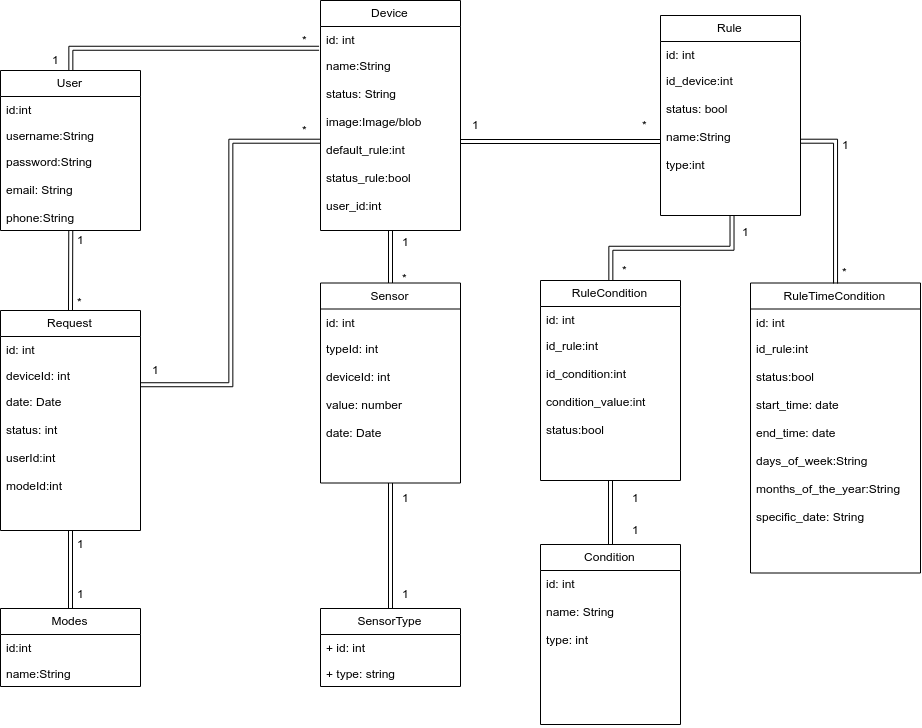
\includegraphics[scale=0.5]{figures/ModelDeDades.png}
\caption{Data model UML}
\end{figure}

\newpage

\section{Product backlog}
%% Product backlog

\newpage

\section{Sprint backlog + dedication to each one}
%% Sprint backlog + dedication to each one

\newpage

\section{Main screens desgin mockup}
%% Main screens desgin mockup

\newpage

\section{Navigation schema between activities}
%% Navigation schema between activities

\newpage

\section{Android prototype}
\subsection{Main screenshot files}
%% Main screenshot files

\newpage

\subsection{Localization}
%% Localization

\newpage

\begin{comment}
\subsection{Brief feasibility study}
\textit{Small estimation of whether the system will be useful for the company and is feasible to be developed under the existing restrictions, in order to determine whether it goes ahead, or is worth investing in a deeper and more serious feasibility study.}
\\\\
The system tries to add an interactive and simple interface to speed up the process of buying and selling tickets at peak times.\\\\
This system has a simple and inexpensive implementation, therefore, the addition of the application to the current working environment would be soon. 
With regard to monetary transactions, we will be able to guarantee optimum security thanks to the use of the *TSL protocol which uses secure communications.\\\\
The system does not foresee problems when using external services such as TicketMaster or the service that processes bank transactions.
\end{comment}
\subsection{Domain}
\textit{Domain Terminology Glossary}\\
\begin{itemize}
\item \textbf{Accessibility}: It is the ability to provide flexibility to accommodate each user's needs and preferences and/or limitations.
\item \textbf{Concurrency}: It is a property of systems in which the processes of a computation are made simultaneously, and can interact among them.
\item \textbf{Interoperability}: It is the capacity of information systems, and by extension of the procedures they support, to share data and enable the exchange of information and knowledge among them.
\item \textbf{Usability}: A measure of the quality of a user's experience when interacting with a product or system.
\item \textbf{User}: A person who uses the system interface.
\end{itemize}

\end{document}